\documentclass[a4paper, smallheadings,english]{scrartcl}

% enable mutated vowls
\usepackage[utf8]{inputenc}

% vector fonts
\usepackage[T1]{fontenc}
% }}}

% {{{ include packages: math, url, fancyhdr
% break up syllables
\usepackage[english,ngerman]{babel}

% add notes to the doc
%\usepackage{marginnote}

% use math
\usepackage{amsmath, amssymb, amsfonts}
\usepackage{array}

% add graphics
\usepackage{lscape, tikz, graphicx}
\usetikzlibrary{backgrounds}

% display urls, code
\usepackage{url, listings}
\lstset{breaklines,commentstyle=\small\ttfamily,basicstyle=\scriptsize\ttfamily}

% enable custom headings
\usepackage{fancyhdr,lastpage,enumerate}
\renewcommand{\labelenumi}{(\roman{enumi})}
% }}}

%{{{ custom headings
%\pagestyle{plain}
% how do I refer to the author, chapter, etc?

\pagestyle{fancy}
\fancyhead[LO]{\Title} %Kopfzeile links
\fancyhead[LE]{\leftmark\rightmark} %Kopfzeile links
\fancyhead[R]{\Author} %Kopfzeile rechts
\fancyfoot[C]{\footnotesize \thepage\ of \pageref{LastPage}}
\fancypagestyle{firststyle}
{
    \renewcommand{\headrulewidth}{0pt}
    \fancyhf{}
    \fancyfoot[C]{\footnotesize \thepage\ of \pageref{LastPage}}
}
% }}}
\setlength{\parskip}{\baselineskip}
\newcommand{\Author}{Jiannan Guo - ICT-Innovation\\Niklas Semmler - ICT-Innovation}
\newcommand{\Title}{Network Management Project}
\newcommand{\note}[1]{\marginnote{\textit{\textbf{#1}} }}
\newcommand{\corr}[2]{\marginnote{\textcolor{red}{#1} }}

\begin{document}
% {{{ Header
\title{\Title}
\author{\Author}
\date{\today}
\maketitle
% }}}
\thispagestyle{firststyle}
\section{Task}
\label{sec:task1}
\subsection{Pseudocode}
The following pseudo code (listing \ref{lst:1}) is inspired by \cite{stadler2012protocols}. To the existing object A a new object Comm was introduced to handle all message exchange.
\begin{lstlisting}[caption={Pseudocode for $\widetilde{f}(t)$ with rate control}, label={lst:1}, numbers=left, frame=single]
messages:
(ResponseTimeArriveMessage, responseTime) # similar to local
(UpdateVector, neighbor) # similar to new and update
(TimeOut, responseTime)

objects and help functions:
A       # storing values for and performing aggregation
Comm    # communication messages
A.aggregate_local       # aggregate local response times for local statistics
A.aggregate_sub_tree    # combine local values with children's for statistics
                        #  of the whole subtree
A.value                 # values of statistics of subtree (including own)
Comm.send_to_self       # send a message to the own node with a delay
Comm.send_to_neighbors  # send to all specified neighbors
Comm.send_to_parent     # send to parent
find_parent             # among neighbors, choose first with minimum level as
                        #  new parent
constants:
DELAY := # fixed time window
INF := # really big number

global variables:
msgBudget = 1

procedure GAP( )
    Neighbors := empty;
    ResponseTimes := empty;

    if v = root then
        level = 0
        parent = 0
    else
        level = INF
        parent = INF
    end if

    A.initiate()
    while true do
        read message;
        switch (message)
            case (ResponseTimeArriveMessage, responseTime)
                ResponseTimes.add(responseTime)
                # to keep only a set of responseTimes in cache
                Comm.send_to_self(DELAY, TimeOut(responseTime))
                A.aggregate_local(ResponseTimes)
                A.aggregate_sub_tree(Neighbors)
            case (UpdateVector, neighbor):
                Neighbors.add(neighbor) 
                (newParent, newLevel) = find_new_parent(Neighbors)
                A.aggregate_sub_tree(Neighbors)
                if (level != newLevel || parent != newParent) then
                    level = newLevel
                    parent = newParent
                    Comm.send_to_neighbors(Neighbors, level, parent, A.value())
                    continue
                end if
            # to keep only a set of responseTimes in cache
            case (TimeOut, responseTime):
                responses.remove(responseTime)
                A.aggregate_local_value(ResponseTimes)
                A.aggregate_sub_tree(Neighbors)
        end switch
        if (msgBudget > 0) then
            Comm.send_to_parent(Neighbors, A.value)
            msgBudget--
        end if
        if (msgBudgetReset) then # waiting for another program to change
            msgBudget = MSG_BUDGET
        endif
    end while
end procedure
procedure ResetMsgBudget()
    msgBudget = 1
end procedure
\end{lstlisting}
\subsection{Implementation Details}
A new base class was implemented which all of the tasks extend: \texttt{peersim.EP2300.vector.GAPNode}. In \texttt{peersim.EP2300.message} three new messages were introduced: \texttt{ResponseTimeArriveMessage}, \texttt{UpdateVector}, \texttt{TimeOut}. The first two roughly equal \texttt{LOCALVAR} and \texttt{UPDATE \& NEW} from the original technical report (see \cite{stadler2012protocols}).

Each node stores all its information on it's neighbors as \texttt{NodeStateVector} in a SortMap named \texttt{neighborList}. Details on the nodes response times are stored in the ArrayList \texttt{requestList}. To focus only on the response times in the current time window, every response time is assigned a time out.

For the implementation with rate control, every message send to the parent will trigger a decrease of the msg budget. As soon as the msg budget is lower or equal to 0, no more messages are sent out. The message budget is reset via a new control \texttt{peersim.EP2300.control.ResetMsgBudget}.
\subsection{Results}
\begin{enumerate}
    \item time series of f(t) and f(t) for r = \{0.2,0.4,0.8\} and \{R1\} from the first 5 minutes
    \item time series of f(t) and f(t) for r = \{0.2,0.4,0.8\} and \{R1\} after the first 5 minutes
    \item trade-off plots for both \{R1,R2\} (and all rate options?? 0.1,0.2,0.4,0.8,1.6)
    \item density plots for r = \{0.2, 0.4, 0.8\} and \{R1,R2\}
\end{enumerate}

\section{Task}
\label{sec:task2}
\subsection{Pseudocode}
In the following the pseudo code for extension 1 is presented. Different to the first task we do not use a message budget (or message rate). Instead an error budget is used. This error budget is assigned to all nodes. Only when the difference of the aggregate of the subtree to the last communicated version of the same exceeds the error budget, a message is sent.

\begin{lstlisting}[caption={Pseudocode for $\widetilde{f}(t)$ with error budget in $P_1$}, label={lst:2}, numbers=left, frame=single]
messages:
[see listing 1]

objects and help functions:
[see listing 1]
A.difference_of_subtree # difference of last communicated value versus current
                        #  communicated value

constants:
DELAY := # fixed time window
INF := # really big number
ERROR_BUDGET = # fix number

global variables:

procedure GAP( )
    Neighbors := empty;
    ResponseTimes := empty;

    if v = root then
        [see listing 1]
    end if

    A.initiate()
    while true do
        read message;
        switch (message)
            [see listing 1]
        end switch
        if (A.difference_of_subtree() > ERROR_BUDGET) then
            Comm.send_to_parent(Neighbors, A.value)
        end if
    end while
end procedure
\end{lstlisting}

\subsection{Implementation Details}
Similar to the difference between the pseudocode of this and task~\ref{sec:task1} the difference in the code is just the replacement of a depletable message budget with a constant error budget.

\section{Task}
\subsection{Pseudocode}
The pseudocode for providing $\widetilde{g}(t)$ under $P_{1}$ is equal to the one provided in section \ref{sec:task2}. The pseudocode for $P_{2}$ is attached below.


\section{foo}

\begin{figure}[h!]
    \begin{center}
        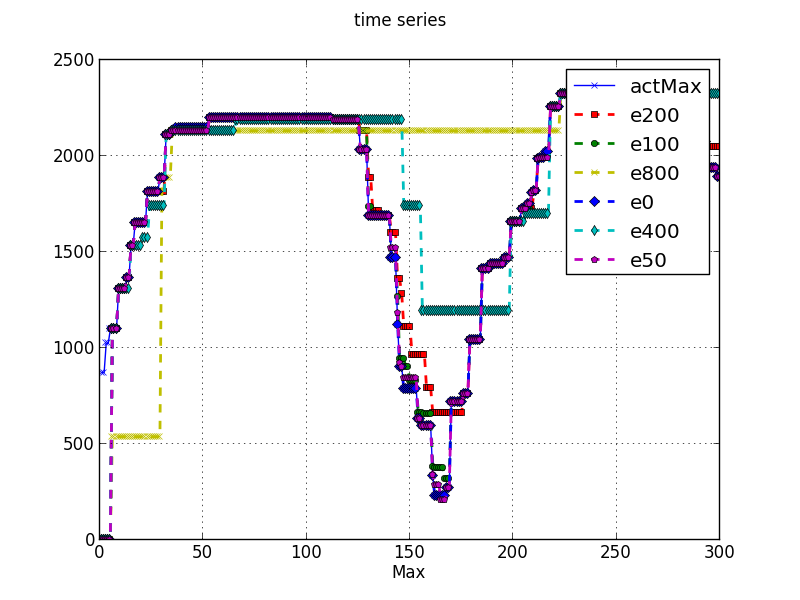
\includegraphics[scale=0.7]{plots/time_series}
    \end{center}
    \caption{Time series plot}
    \label{fig:ts}
\end{figure}
\begin{figure}[h!]
    \begin{center}
        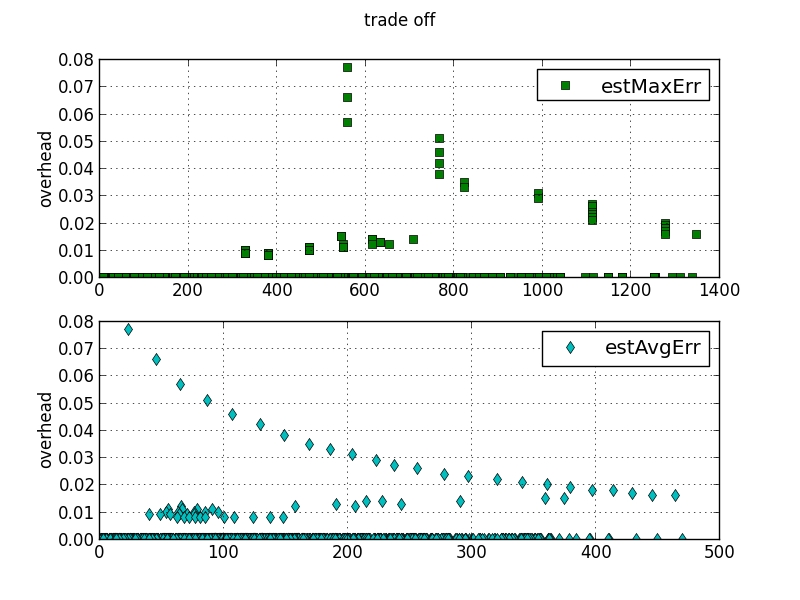
\includegraphics[scale=0.7]{plots/trade_off}
    \end{center}
    \caption{Trade off plot}
    \label{fig:to}
\end{figure}
\begin{figure}[h!]
    \begin{center}
        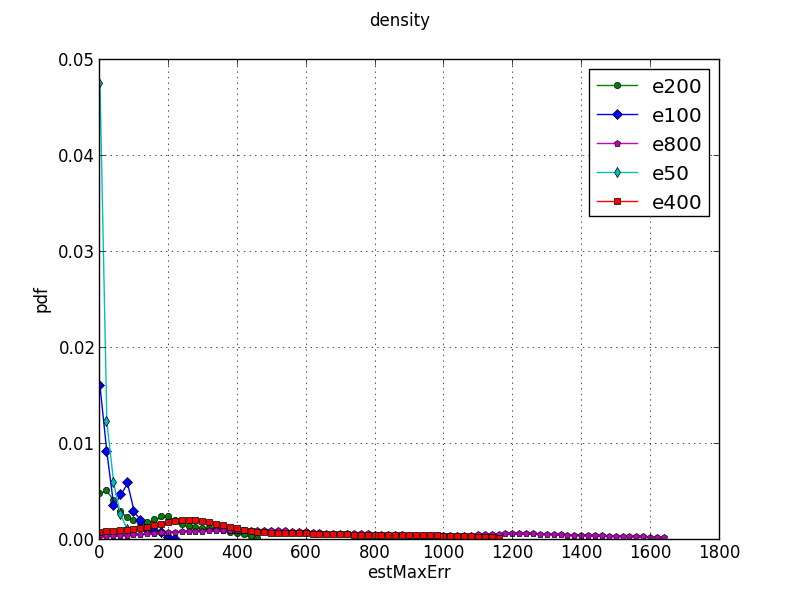
\includegraphics[scale=0.7]{plots/pdf_of_error}
    \end{center}
    \caption{PDF plot}
    \label{fig:pdf}
\end{figure}

\begin{itemize}
    \item compare performance for $R_1, R_2$
    \begin{itemize}
        \item time series of f~(t) and f(t) for r = \{ 0.2, 0.4, 0.8 \} amd \{$R_1$, $R_2$\} from the first 5 min
        \item trade off plot for $R_1, R_2$
        \item density plot for r = \{ 0.2, 0.4, 0.8 \} and \{$R_1$, $R_2$\}
    \end{itemize}
\end{itemize}

\section{Task II}
\begin{itemize}
    \item pseudo code!
    \item implementation details
    \item compare performance for $R_1, R_2$
    \begin{itemize}
        \item time series of f~(t) and f(t) for r = \{ 0.2, 0.1, 0.05, 0.025, \} amd \{$R_1$, $R_2$\} from the first 5 min
        \item trade off plot for $R_1, R_2$
        \item density plot for r = \{ 0.1, 0.05, 0.025 \} and \{$R_1$, $R_2$\}
    \end{itemize}
\end{itemize}

\section{Task III}
\begin{itemize}
    \item pseudo code!
    \item implementation details
    \item compare performance for $R_1, R_2$
    \begin{itemize}
        \item time series of f~(t) and f(t) for r = \{ 0.2, 0.1, 0.05, 0.025, \} amd \{$R_1$, $R_2$\} from the first 5 min
        \item trade off plot for $R_1, R_2$
        \item density plot for r = \{ 0.1, 0.05, 0.025 \} and \{$R_1$, $R_2$\}
    \end{itemize}
\end{itemize}

\section{Summary}
\begin{itemize}
    \item Compare TaskI, II, III
    \item Compare $R_1, R_2$ globally
\end{itemize}
\bibliographystyle{ieeetr}
\bibliography{report}

\begin{appendix}
\section{Calculations}
\subsection{Distribution of error budget in aggregation via average}
\textbf{Definitions}\\
\begin{tabular}{>{$}l<{$} >{$}l<{$} >{$}l<{$}}
\epsilon &:= \text{Local error budget of a node} &\ge 0\\
\Phi &:= \text{Overall error budget} &\ge 0\\
X &:= \text{Previous sum of the response times in subtree} &\ge 0 \\
Y &:= \text{Previous number of requests in subtree} &\ge 0\\
\Delta Y &:= \text{Number of newly arrived reqeusts in subtree} &\ge 0\\
\end{tabular}
\textbf{Aim}\\
It is the aim of this proof to show how the error budget $\epsilon$ for every node $i$ can be maximized ($\epsilon_{max}$) while keeping the global error budget $\Phi$ constant. The aggregation operation in this case is averaging of the response times of all requests.

\noindent \textbf{Proof}\\
\begin{align}
\Phi & \ge \left| \frac{X + \Delta Y \cdot \epsilon}{Y+\Delta Y}-\frac{X}{Y}\right| \label{ineq:phi}\\
\epsilon & \le
\begin{cases}
\frac{\left(Y+\Delta Y\right)\Phi}{\Delta Y}+\frac{X}{Y} & \text{if } Y \neq 0\\
\Phi & \text{if } Y = 0
\end{cases}
\label{ineq:eps}\\ \notag
\end{align}
The task to find maximum value of $\epsilon$ can be transformed to finding minimum value of the right side of inequation \ref{ineq:eps}.

\noindent When $Y \neq 0$ we have
\[\frac{Y+\Delta Y}{\Delta Y} > 1, \frac{X}{Y} \ge 0\]
thus
\[\frac{\left(Y + \Delta Y\right) \Phi}{\Delta Y} + \frac{X}{Y} \ge \Phi\]
When  $Y = 0$, the minimum of right side is $\Phi$, thus the minimum value of right side of inequeation is $\Phi$. 

\noindent It follows $\epsilon_{max} = \Phi$.
\newpage
\subsection{Distribution of error budget based on message rate}
\textbf{Definitions}\\
Other than the definitions for problem 3a:\\
\begin{tabular}{>{$}l<{$} >{$}l<{$} >{$}l<{$}}
\alpha &:= \text{Factor of relation between error budget and request rate} &\ge 0\\
\delta &:= \text{Number of newly arrived requests in a node per time unit} &\\
\end{tabular}
\textbf{Aim}\\
The aim of this proof is to find the maximum factor $\alpha$ relating the request rate $\delta_i$ with the the error budget $\epsilon$.

\noindent \textbf{Proof}\\
For every node $i$ with the $S(i)$ denoting all nodes that are direct children of $i$ in the network and i itself.
\begin{align}
\left|
\begin{array}{ll}
\Phi \ge& \frac{X + \sum_{j \in S(i)} \epsilon_j \cdot \delta_j}{Y + \sum_{j \in S(i)} \delta_j} - \frac{X}{Y}\\
\epsilon_i =& \alpha \cdot \delta_i
\end{array}
\right|\\\notag
\end{align}
Applying the same schema of problem 3a, we can have\\
\begin{align}
\Phi &\ge \frac{\sum_{j \in S(i)} \epsilon_j \cdot \delta_j}{\sum_{j \in S(i)} \delta_j}\\\notag
\end{align}
substitute $\epsilon_i$ with $\alpha\cdot\delta_i$, we have:\\
\begin{align}
\Phi &\ge \frac{\sum_{j \in S(i)} \alpha \cdot \delta_j^2}{\sum_{j \in S(i)} \delta_j}\\
\alpha &\le \frac{\sum_{j \in S(i)} \delta_j}{\sum_{j \in S(i)} \delta_j^2} \cdot \Phi\\\notag
\end{align}
Hence the max factor is:\\
\begin{align}
\alpha_{max} &= \frac{\sum_{j \in S(i)} \delta_j}{\sum_{j \in S(i)} \delta_j^2} \cdot \Phi\\\notag
\end{align}

\noindent Thus error budget for node i is $\alpha_{max} \cdot \delta_i = \delta_i \frac{\sum_{j \in S(i)} \delta_j}{\sum_{j \in S(i)} \delta_j^2} \cdot \Phi$
\end{appendix}
\end{document}
